%**************************************************************************************
% License:
% CC BY-NC-SA 4.0 (http://creativecommons.org/licenses/by-nc-sa/4.0/)
%**************************************************************************************

\documentclass[aspectratio=169]{beamer}

\mode<presentation> {
	\usetheme{Madrid}

	% Burnt orange
	\definecolor{burntorange}{rgb}{0.8, 0.33, 0.0}
	\colorlet{beamer@blendedblue}{burntorange}
	% Pale yellow
	\definecolor{paleyellow}{rgb}{1.0, 1.0, 0.953}
	\setbeamercolor{background canvas}{bg=paleyellow}
	% Secondary and tertiary palette
	\setbeamercolor*{palette secondary}{use=structure,fg=white,bg=burntorange!80!black}
	\setbeamercolor*{palette tertiary}{use=structure,fg=white,bg=burntorange!60!black}

	% Remove navigation symbols
	\setbeamertemplate{navigation symbols}{}
}

\usepackage{amsmath,amssymb,amsthm}
\usepackage{bm}
\usepackage{booktabs}
\usepackage{graphicx}
\usepackage[labelsep=space,tableposition=top]{caption}
\renewcommand{\figurename}{Fig.}
\usepackage{caption,subcaption}
\usepackage{xcolor}
\usepackage{transparent}
\usepackage{hyperref}
\usepackage{tikz}
\usepackage{listings}
\usetikzlibrary{shapes,arrows,positioning,calc}
\usepackage{pgfplots}
\pgfplotsset{compat=1.17}

% Define math operators
\DeclareMathOperator*{\argmin}{arg\,min}
\DeclareMathOperator*{\argmax}{arg\,max}
\newcommand{\norm}[1]{\left\lVert#1\right\rVert}

% Code listing style
\lstset{
    language=Python,
    basicstyle=\tiny\ttfamily,
    keywordstyle=\color{blue},
    commentstyle=\color{gray},
    stringstyle=\color{green!70!black},
    showstringspaces=false,
    frame=single,
    breaklines=true,
    numbers=left,
    numberstyle=\tiny
}

\AtBeginSection[]{
	\begin{frame}{Outline}
		\tableofcontents[
		currentsection,      % highlight the current section
		hideallsubsections   % show only section titles
		]
	\end{frame}
}

%----------------------------------------------------------------------------------------
%	TITLE PAGE
%----------------------------------------------------------------------------------------
\title[Exploratory Data Analysis]{Exploratory Data Analysis for Geotechnical Engineering}
\author{Krishna Kumar and Ellen Rathje} % name
\institute[UT Austin] % institution
{
University of Texas at Austin \\
\medskip
\textit{
  \url{krishnak@utexas.edu}} % Your email address
}
\date{} % Date, can be changed to a custom date

\begin{document}

\begin{frame}
\titlepage % title page as the first slide
\end{frame}

\begin{frame}
 \frametitle{Overview}
 \tableofcontents
\end{frame}

%----------------------------------------------------------------------------------------
% slides
%----------------------------------------------------------------------------------------

\section{Introduction to EDA}

%------------------------------------------------
\begin{frame}
\frametitle{Learning Objectives}

\begin{itemize}
    \item Understand the importance of EDA in geotechnical machine learning
    \item Learn systematic approaches to data exploration and quality assessment
    \item Master techniques for detecting and handling missing data and outliers
    \item Apply statistical methods to understand feature distributions and relationships
    \item Make informed decisions about data preprocessing and feature engineering
\end{itemize}

\vspace{1cm}
\centering
\href{https://colab.research.google.com/github/kks32-courses/ai-geotech/blob/main/docs/00-mlp-dtree/00-eda-liquefaction.ipynb}{\beamergotobutton{Open Notebook: EDA Liquefaction}}

\end{frame}

%------------------------------------------------
\begin{frame}
\frametitle{What is Exploratory Data Analysis?}

\begin{block}{Definition}
EDA is the critical process of performing initial investigations on data to discover patterns, spot anomalies, test hypotheses, and check assumptions through summary statistics and graphical representations.
\end{block}

\vspace{0.5cm}

\textbf{Why EDA Matters in Geotechnical Engineering:}
\begin{itemize}
    \item \textbf{Data Quality}: Identify measurement errors, missing values, outliers
    \item \textbf{Physical Validation}: Ensure data aligns with engineering knowledge
    \item \textbf{Feature Understanding}: Discover which parameters affect outcomes
    \item \textbf{Model Preparation}: Inform preprocessing and feature engineering decisions
    \item \textbf{Risk Mitigation}: Catch issues before they propagate to models
\end{itemize}

\end{frame}

%------------------------------------------------
\begin{frame}
\frametitle{The EDA Workflow}

\begin{figure}[ht]
	\centering
	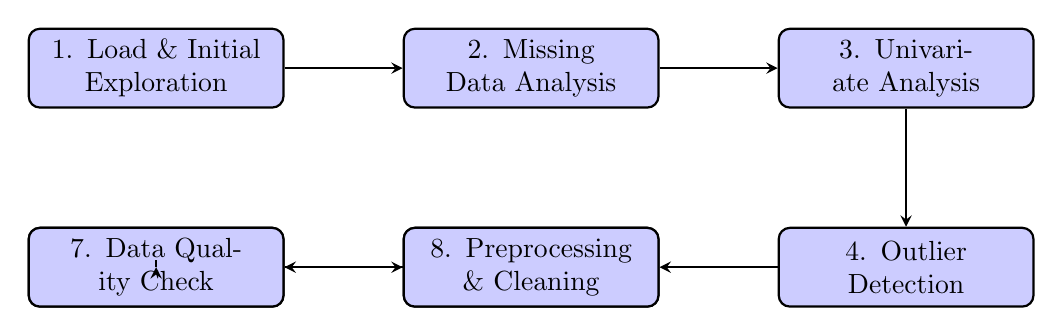
\begin{tikzpicture}[node distance=1.5cm, auto, thick,
		box/.style={rectangle, draw, fill=blue!20, text width=3cm, text centered, rounded corners, minimum height=1cm},
		arrow/.style={->, >=stealth, thick}]

		\node [box] (load) {1. Load \& Initial Exploration};
		\node [box, right=of load] (missing) {2. Missing Data Analysis};
		\node [box, right=of missing] (univariate) {3. Univariate Analysis};
		\node [box, below=of univariate] (outliers) {4. Outlier Detection};
		\node [box, left=of outliers] (bivariate) {5. Bivariate Analysis};
		\node [box, left=of bivariate] (multivariate) {6. Multivariate Analysis};
		\node [box, below=of load] (quality) {7. Data Quality Check};
		\node [box, right=of quality] (clean) {8. Preprocessing \& Cleaning};

		\draw [arrow] (load) -- (missing);
		\draw [arrow] (missing) -- (univariate);
		\draw [arrow] (univariate) -- (outliers);
		\draw [arrow] (outliers) -- (bivariate);
		\draw [arrow] (bivariate) -- (multivariate);
		\draw [arrow] (multivariate) -- (quality);
		\draw [arrow] (quality) -- (clean);

	\end{tikzpicture}
\end{figure}

\textbf{Key Principle}: Iterate through these steps; EDA is not strictly linear!

\end{frame}

%------------------------------------------------
\begin{frame}
\frametitle{Case Study: Liquefaction and Lateral Spreading}

\begin{columns}[T]
    \begin{column}{0.5\textwidth}
        \textbf{The Problem:}
        \begin{itemize}
            \item Soil liquefaction during earthquakes
            \item Lateral spreading on gently sloping ground
            \item Sites with >0.3m displacement = failure
        \end{itemize}

        \vspace{0.3cm}

        \textbf{Dataset:} Durante \& Rathje (2021)
        \begin{itemize}
            \item 7,291 observations from Christchurch
            \item Binary classification problem
            \item Real geotechnical measurements
        \end{itemize}
    \end{column}
    \begin{column}{0.5\textwidth}
        \textbf{Key Features:}
        \begin{itemize}
            \item \textbf{GWD (m)}: Ground water depth
            \item \textbf{L (km)}: Distance to free face
            \item \textbf{Slope (\%)}: Ground slope angle
            \item \textbf{PGA (g)}: Peak ground acceleration
            \item \textbf{Target}: 0 = No spreading, 1 = Spreading
        \end{itemize}

        \vspace{0.3cm}

        This dataset is perfect for demonstrating EDA techniques applicable to any geotechnical problem!
    \end{column}
\end{columns}

\end{frame}

\section{Data Understanding}

%------------------------------------------------
\begin{frame}
\frametitle{Initial Data Exploration}

\textbf{First Questions to Ask:}
\begin{itemize}
    \item How many samples do we have?
    \item What are the features (columns)?
    \item What are the data types?
    \item Are there any obvious issues?
\end{itemize}

\vspace{0.5cm}

\textbf{Essential Commands (Pandas):}
\begin{itemize}
    \item \texttt{df.head()} - View first few rows
    \item \texttt{df.info()} - Data types and non-null counts
    \item \texttt{df.describe()} - Statistical summary
    \item \texttt{df.shape} - Dataset dimensions
\end{itemize}

\end{frame}

%------------------------------------------------
\begin{frame}[fragile]
\frametitle{Statistical Summaries}

\begin{block}{Key Statistics to Examine}
\begin{itemize}
    \item \textbf{Count}: Number of non-null observations
    \item \textbf{Mean vs. Median}: Indicates distribution symmetry
    \item \textbf{Std (Standard Deviation)}: Measure of spread
    \item \textbf{Min/Max}: Range and potential outliers
    \item \textbf{Quartiles (25\%, 50\%, 75\%)}: Distribution shape
\end{itemize}
\end{block}

\vspace{0.3cm}

\textbf{Geotechnical Interpretation Example:}
\begin{itemize}
    \item GWD mean = 2.1m, median = 2.0m → Fairly symmetric
    \item GWD range: 0.2m to 4.5m → Typical for liquefaction sites
    \item PGA range: 0.35g to 0.60g → Moderate to strong shaking
\end{itemize}

\end{frame}

%------------------------------------------------
\begin{frame}
\frametitle{Understanding Data Types}

\begin{columns}[T]
    \begin{column}{0.5\textwidth}
        \textbf{Continuous Variables:}
        \begin{itemize}
            \item Measurements on a scale
            \item Can take any value in range
            \item Examples: GWD, PGA, Slope
        \end{itemize}

        \textbf{Analysis Methods:}
        \begin{itemize}
            \item Histograms, box plots
            \item Mean, median, std
            \item Correlation analysis
        \end{itemize}
    \end{column}
    \begin{column}{0.5\textwidth}
        \textbf{Categorical Variables:}
        \begin{itemize}
            \item Distinct groups/categories
            \item Limited set of values
            \item Examples: Soil type, Target class
        \end{itemize}

        \textbf{Analysis Methods:}
        \begin{itemize}
            \item Bar charts, count plots
            \item Mode, frequency tables
            \item Chi-square tests
        \end{itemize}
    \end{column}
\end{columns}

\vspace{0.5cm}

\textbf{Important}: Different data types require different analysis techniques and preprocessing!

\end{frame}

%------------------------------------------------
\begin{frame}
\frametitle{Visualizing Distributions}

\begin{columns}[T]
    \begin{column}{0.33\textwidth}
        \textbf{Histograms:}
        \begin{itemize}
            \item Show frequency distribution
            \item Reveal shape and spread
            \item Identify modality
            \item Spot gaps/clusters
        \end{itemize}
    \end{column}
    \begin{column}{0.33\textwidth}
        \textbf{Box Plots:}
        \begin{itemize}
            \item Display quartiles
            \item Identify outliers
            \item Compare distributions
            \item Show range compactly
        \end{itemize}
    \end{column}
    \begin{column}{0.34\textwidth}
        \textbf{KDE Plots:}
        \begin{itemize}
            \item Smooth density estimate
            \item Better for comparison
            \item Shows distribution shape
            \item Continuous representation
        \end{itemize}
    \end{column}
\end{columns}

\vspace{0.5cm}

\textbf{Tip}: Use multiple visualization types to get complete understanding!

\end{frame}

\section{Missing Data Analysis}

%------------------------------------------------
\begin{frame}
\frametitle{Types of Missing Data}

\begin{block}{Three Categories of Missingness}
\begin{enumerate}
    \item \textbf{MCAR (Missing Completely At Random):}
    \begin{itemize}
        \item No pattern to missingness
        \item Unrelated to any variables
        \item Safest to remove or impute
    \end{itemize}

    \item \textbf{MAR (Missing At Random):}
    \begin{itemize}
        \item Missingness related to observed variables
        \item Example: Deep GWD measurements missing (too expensive)
        \item Requires careful imputation
    \end{itemize}

    \item \textbf{MNAR (Missing Not At Random):}
    \begin{itemize}
        \item Missingness related to the missing value itself
        \item Example: Failed tests not recorded
        \item Most challenging to handle
    \end{itemize}
\end{enumerate}
\end{block}

\end{frame}

%------------------------------------------------
\begin{frame}
\frametitle{Detecting Missing Data}

\textbf{Detection Methods:}
\begin{itemize}
    \item \texttt{df.isnull().sum()} - Count missing per column
    \item \texttt{df.isnull().sum() / len(df)} - Percentage missing
    \item Heatmaps - Visualize missing patterns across dataset
    \item Correlation of missingness - Do variables tend to be missing together?
\end{itemize}

\vspace{0.5cm}

\textbf{Key Questions:}
\begin{itemize}
    \item What percentage of data is missing?
    \item Is missingness random or patterned?
    \item Which features are most affected?
    \item Can we infer why data is missing?
\end{itemize}

\end{frame}

%------------------------------------------------
\begin{frame}
\frametitle{Handling Missing Data: Strategies}

\begin{columns}[T]
    \begin{column}{0.5\textwidth}
        \textbf{Deletion Methods:}
        \begin{itemize}
            \item \textbf{Listwise}: Remove entire row
            \begin{itemize}
                \item Use if $<5\%$ missing and MCAR
                \item Simple but loses data
            \end{itemize}
            \item \textbf{Pairwise}: Use available data
            \begin{itemize}
                \item Maximize data usage
                \item Can cause inconsistencies
            \end{itemize}
        \end{itemize}
    \end{column}
    \begin{column}{0.5\textwidth}
        \textbf{Imputation Methods:}
        \begin{itemize}
            \item \textbf{Mean/Median/Mode}
            \begin{itemize}
                \item Simple and fast
                \item Reduces variance
            \end{itemize}
            \item \textbf{Domain Knowledge}
            \begin{itemize}
                \item Use engineering judgment
                \item Most appropriate for geotechnics
            \end{itemize}
            \item \textbf{Advanced (KNN, MICE)}
            \begin{itemize}
                \item More accurate
                \item Computationally expensive
            \end{itemize}
        \end{itemize}
    \end{column}
\end{columns}

\end{frame}

%------------------------------------------------
\begin{frame}
\frametitle{Geotechnical Considerations for Missing Data}

\textbf{Example Scenarios:}

\begin{enumerate}
    \item \textbf{Missing GWD measurements:}
    \begin{itemize}
        \item Could indicate very deep water table (not liquefaction-prone)
        \item Consider: Keep as separate category vs. Impute with regional average
        \item Engineering judgment: Sites without GWD likely low risk
    \end{itemize}

    \item \textbf{Missing SPT N-values:}
    \begin{itemize}
        \item Might correlate with CPT data if available
        \item Use empirical correlations from literature
        \item Regional geological data can inform imputation
    \end{itemize}

    \item \textbf{Missing laboratory test results:}
    \begin{itemize}
        \item Often for preliminary boring logs
        \item Use site characterization to estimate
        \item Consider similar soil types nearby
    \end{itemize}
\end{enumerate}

\textbf{Key Principle}: Always apply geotechnical engineering knowledge when handling missing data!

\end{frame}

\section{Outlier Analysis}

%------------------------------------------------
\begin{frame}
\frametitle{What Are Outliers?}

\begin{block}{Definition}
Outliers are data points that deviate significantly from other observations. They can arise from:
\begin{itemize}
    \item Measurement or recording errors
    \item Extreme but valid events (e.g., major earthquakes)
    \item Natural variability in geological conditions
    \item Data processing errors
\end{itemize}
\end{block}

\vspace{0.5cm}

\textbf{Why Outliers Matter:}
\begin{itemize}
    \item Can severely bias model training
    \item May represent critical edge cases
    \item Affect statistical measures (mean, std)
    \item Some models robust to outliers (trees), others sensitive (linear, neural nets)
\end{itemize}

\end{frame}

%------------------------------------------------
\begin{frame}
\frametitle{Detection Method 1: Box Plot and IQR}

\begin{columns}[T]
    \begin{column}{0.5\textwidth}
        \textbf{Interquartile Range (IQR) Method:}

        \begin{equation*}
        \begin{aligned}
        IQR &= Q_3 - Q_1 \\
        \text{Lower Bound} &= Q_1 - 1.5 \times IQR \\
        \text{Upper Bound} &= Q_3 + 1.5 \times IQR
        \end{aligned}
        \end{equation*}

        Points outside these bounds are outliers.

        \vspace{0.3cm}

        \textbf{Pros:}
        \begin{itemize}
            \item Simple and intuitive
            \item Visual interpretation
            \item Robust to distribution shape
        \end{itemize}
    \end{column}
    \begin{column}{0.5\textwidth}
        \textbf{Cons:}
        \begin{itemize}
            \item Fixed threshold (1.5× IQR)
            \item Univariate only
            \item May flag valid extremes
        \end{itemize}

        \vspace{0.3cm}

        \textbf{Box Plot Components:}
        \begin{itemize}
            \item Box: IQR (Q1 to Q3)
            \item Line in box: Median (Q2)
            \item Whiskers: 1.5× IQR
            \item Points beyond: Outliers
        \end{itemize}
    \end{column}
\end{columns}

\end{frame}

%------------------------------------------------
\begin{frame}
\frametitle{Detection Method 2: Z-Score}

\textbf{Z-Score (Standard Score):}
\begin{equation*}
z = \frac{x - \mu}{\sigma}
\end{equation*}

\begin{itemize}
    \item Measures how many standard deviations from the mean
    \item Common threshold: $|z| > 3$ (99.7\% of data within ±3σ for normal distribution)
    \item Assumes approximately normal distribution
\end{itemize}

\vspace{0.5cm}

\begin{columns}[T]
    \begin{column}{0.5\textwidth}
        \textbf{Pros:}
        \begin{itemize}
            \item Well-understood statistical basis
            \item Adjustable threshold
            \item Works with normalized data
        \end{itemize}
    \end{column}
    \begin{column}{0.5\textwidth}
        \textbf{Cons:}
        \begin{itemize}
            \item Sensitive to mean and std
            \item Assumes normal distribution
            \item Affected by outliers themselves
            \item Univariate only
        \end{itemize}
    \end{column}
\end{columns}

\end{frame}

%------------------------------------------------
\begin{frame}
\frametitle{Detection Method 3: Isolation Forest}

\begin{columns}[T]
    \begin{column}{0.5\textwidth}
        \textbf{Machine Learning Approach:}
        \begin{itemize}
            \item Isolates anomalies using random partitioning
            \item Anomalies are easier to isolate (require fewer splits)
            \item Works in multivariate space
            \item No distribution assumptions
        \end{itemize}

        \vspace{0.3cm}

        \textbf{How it works:}
        \begin{enumerate}
            \item Build random decision trees
            \item Calculate average path length
            \item Shorter paths → Outliers
        \end{enumerate}
    \end{column}
    \begin{column}{0.5\textwidth}
        \textbf{Pros:}
        \begin{itemize}
            \item Multivariate detection
            \item Handles complex patterns
            \item Scalable to large datasets
            \item No parameter tuning needed
        \end{itemize}

        \vspace{0.3cm}

        \textbf{Cons:}
        \begin{itemize}
            \item Less interpretable
            \item Requires setting contamination rate
            \item May miss subtle outliers
        \end{itemize}
    \end{column}
\end{columns}

\vspace{0.3cm}

\textbf{Typical usage:} \texttt{IsolationForest(contamination=0.1)} assumes 10\% outliers

\end{frame}

%------------------------------------------------
\begin{frame}
\frametitle{Geotechnical Perspective on Outliers}

\begin{block}{Critical Distinction}
\textbf{Error vs. Extreme Event}: Not all outliers should be removed!
\end{block}

\vspace{0.3cm}

\textbf{Physical Plausibility Checks:}

\begin{table}
\centering
\begin{tabular}{lll}
\toprule
\textbf{Feature} & \textbf{Typical Range} & \textbf{Red Flags} \\
\midrule
GWD & 0 - 5m & Negative values, >20m \\
PGA & 0.1g - 1.0g & Negative, >2.0g (rare) \\
Slope & 0 - 30\% & Negative values \\
Distance & 0 - 5km & Negative values \\
\bottomrule
\end{tabular}
\end{table}

\vspace{0.3cm}

\textbf{Decision Framework:}
\begin{itemize}
    \item \textcolor{red}{\textbf{Remove}}: Physically impossible, obvious errors
    \item \textcolor{green}{\textbf{Keep}}: Valid extreme events, critical edge cases
    \item \textcolor{orange}{\textbf{Investigate}}: Borderline cases, consult domain experts
\end{itemize}

\end{frame}

%------------------------------------------------
\begin{frame}
\frametitle{Outlier Decision Framework}

\begin{figure}
\centering
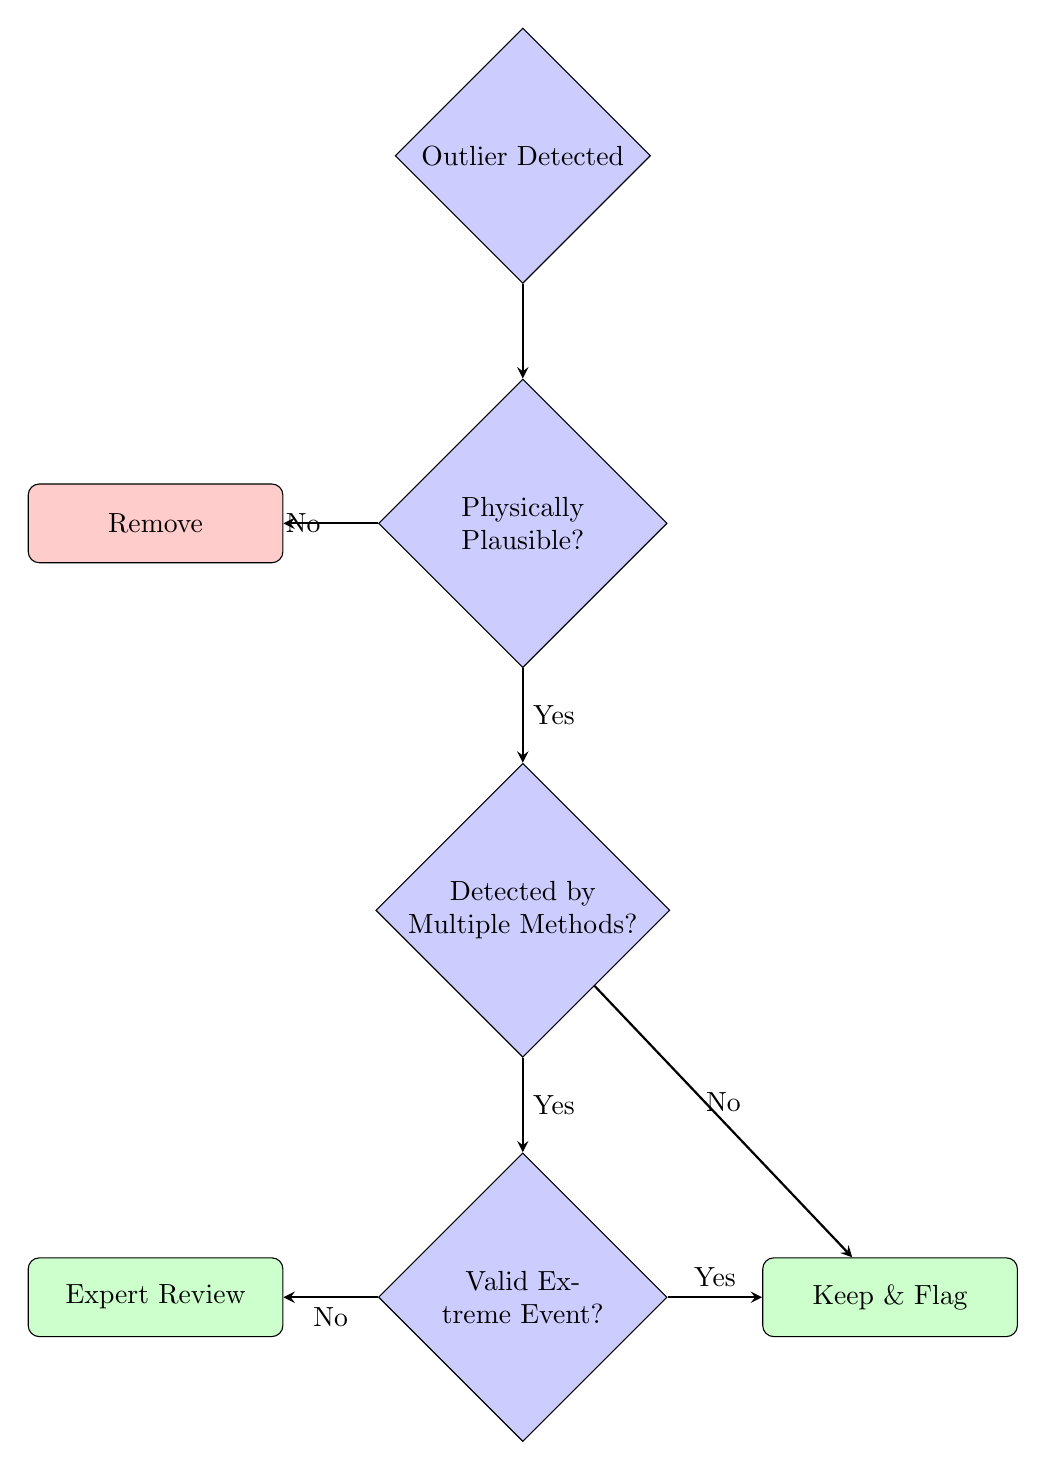
\begin{tikzpicture}[
    node distance=1.2cm,
    decision/.style={diamond, draw, fill=blue!20, text width=3cm, text centered, inner sep=0pt, minimum height=1.5cm},
    action/.style={rectangle, draw, fill=green!20, text width=3cm, text centered, rounded corners, minimum height=1cm},
    reject/.style={rectangle, draw, fill=red!20, text width=3cm, text centered, rounded corners, minimum height=1cm},
    arrow/.style={->, >=stealth, thick}
]

\node [decision] (detect) {Outlier Detected};
\node [decision, below=of detect] (physical) {Physically Plausible?};
\node [reject, left=of physical] (remove) {Remove};
\node [decision, below=of physical] (multiple) {Detected by Multiple Methods?};
\node [decision, below=of multiple] (extreme) {Valid Extreme Event?};
\node [action, right=of extreme] (keep) {Keep \& Flag};
\node [action, left=of extreme] (review) {Expert Review};

\draw [arrow] (detect) -- (physical);
\draw [arrow] (physical) -- node[left] {No} (remove);
\draw [arrow] (physical) -- node[right] {Yes} (multiple);
\draw [arrow] (multiple) -- node[right] {Yes} (extreme);
\draw [arrow] (multiple) -- node[above] {No} (keep);
\draw [arrow] (extreme) -- node[above] {Yes} (keep);
\draw [arrow] (extreme) -- node[below] {No} (review);

\end{tikzpicture}
\end{figure}

\end{frame}

\section{Univariate Analysis}

%------------------------------------------------
\begin{frame}
\frametitle{Distribution Analysis}

\textbf{Key Metrics for Continuous Variables:}

\begin{columns}[T]
    \begin{column}{0.5\textwidth}
        \textbf{Central Tendency:}
        \begin{itemize}
            \item \textbf{Mean}: Average value
            \item \textbf{Median}: Middle value (50th percentile)
            \item \textbf{Mode}: Most frequent value
        \end{itemize}

        \vspace{0.3cm}

        \textbf{When mean ≠ median:}
        \begin{itemize}
            \item Distribution is skewed
            \item Outliers present
            \item Consider transformation
        \end{itemize}
    \end{column}
    \begin{column}{0.5\textwidth}
        \textbf{Spread:}
        \begin{itemize}
            \item \textbf{Range}: Max - Min
            \item \textbf{Std Dev}: Average deviation from mean
            \item \textbf{Variance}: Square of std dev
            \item \textbf{IQR}: Q3 - Q1 (robust measure)
        \end{itemize}

        \vspace{0.3cm}

        \textbf{Percentiles:}
        \begin{itemize}
            \item Q1 (25\%), Q2 (50\%), Q3 (75\%)
            \item Useful for understanding distribution shape
        \end{itemize}
    \end{column}
\end{columns}

\end{frame}

%------------------------------------------------
\begin{frame}
\frametitle{Skewness and Kurtosis}

\begin{columns}[T]
    \begin{column}{0.5\textwidth}
        \textbf{Skewness}: Measures asymmetry

        \begin{equation*}
        \text{Skewness} = \frac{E[(X-\mu)^3]}{\sigma^3}
        \end{equation*}

        \begin{itemize}
            \item Skew = 0: Symmetric (normal)
            \item Skew > 0: Right-skewed (long right tail)
            \item Skew < 0: Left-skewed (long left tail)
        \end{itemize}

        \vspace{0.3cm}

        \textbf{Example:} PGA often right-skewed (rare extreme values)
    \end{column}
    \begin{column}{0.5\textwidth}
        \textbf{Kurtosis}: Measures tail heaviness

        \begin{equation*}
        \text{Kurtosis} = \frac{E[(X-\mu)^4]}{\sigma^4} - 3
        \end{equation*}

        \begin{itemize}
            \item Kurt ≈ 0: Normal distribution
            \item Kurt > 0: Heavy tails (leptokurtic)
            \item Kurt < 0: Light tails (platykurtic)
        \end{itemize}

        \vspace{0.3cm}

        \textbf{Implication:} High kurtosis indicates outliers/extreme events
    \end{column}
\end{columns}

\vspace{0.5cm}

\textbf{For Modeling:} Tree-based models handle skewness well; neural networks may benefit from transformation (log, sqrt)

\end{frame}

%------------------------------------------------
\begin{frame}
\frametitle{Normality Assessment}

\textbf{Why Test for Normality?}
\begin{itemize}
    \item Many statistical tests assume normal distribution
    \item Helps choose appropriate preprocessing
    \item Informs model selection
\end{itemize}

\vspace{0.5cm}

\textbf{Visual Methods:}
\begin{itemize}
    \item Histogram with normal curve overlay
    \item Q-Q plot (quantile-quantile)
    \item KDE plot comparison
\end{itemize}

\vspace{0.5cm}

\textbf{Statistical Tests:}
\begin{itemize}
    \item Shapiro-Wilk test (small samples)
    \item Kolmogorov-Smirnov test
    \item Anderson-Darling test
\end{itemize}

\vspace{0.3cm}

\textbf{Note:} Geotechnical data often not normally distributed—that's okay! Just need to be aware.

\end{frame}

\section{Bivariate \& Multivariate Analysis}

%------------------------------------------------
\begin{frame}
\frametitle{Correlation Analysis}

\textbf{Pearson Correlation Coefficient:}
\begin{equation*}
r = \frac{\sum (x_i - \bar{x})(y_i - \bar{y})}{\sqrt{\sum (x_i - \bar{x})^2 \sum (y_i - \bar{y})^2}}
\end{equation*}

\begin{itemize}
    \item Range: -1 to +1
    \item $r > 0$: Positive correlation (both increase together)
    \item $r < 0$: Negative correlation (one increases, other decreases)
    \item $|r| < 0.3$: Weak; $0.3 \leq |r| < 0.7$: Moderate; $|r| \geq 0.7$: Strong
\end{itemize}

\vspace{0.5cm}

\textbf{Important Caveats:}
\begin{itemize}
    \item Measures \textit{linear} relationships only
    \item Correlation ≠ Causation
    \item Outliers can distort correlation
    \item Use heatmaps for visualizing correlation matrices
\end{itemize}

\end{frame}

%------------------------------------------------
\begin{frame}
\frametitle{Multicollinearity}

\begin{block}{Definition}
Multicollinearity occurs when two or more features are highly correlated with each other.
\end{block}

\vspace{0.3cm}

\textbf{Why It Matters:}
\begin{itemize}
    \item Makes it hard to assess individual feature importance
    \item Increases variance in coefficient estimates (linear models)
    \item Can cause numerical instability
    \item Tree-based models handle it well; linear models struggle
\end{itemize}

\vspace{0.3cm}

\textbf{Detection:}
\begin{itemize}
    \item Correlation matrix: Look for $|r| > 0.7$
    \item Variance Inflation Factor (VIF): VIF > 10 indicates problem
\end{itemize}

\vspace{0.3cm}

\textbf{Solutions:}
\begin{itemize}
    \item Remove one of correlated features
    \item Use PCA to create uncorrelated components
    \item Regularization (Ridge, Lasso) for linear models
\end{itemize}

\end{frame}

%------------------------------------------------
\begin{frame}
\frametitle{Feature-Target Relationships}

\textbf{For Classification Tasks:}

\begin{columns}[T]
    \begin{column}{0.5\textwidth}
        \textbf{Visual Methods:}
        \begin{itemize}
            \item Box plots by class
            \item Violin plots
            \item Density plots colored by class
            \item Scatter plots with class colors
        \end{itemize}

        \textbf{Goal:} See if feature distributions differ between classes
    \end{column}
    \begin{column}{0.5\textwidth}
        \textbf{Statistical Tests:}
        \begin{itemize}
            \item t-test (parametric, 2 classes)
            \item ANOVA (parametric, >2 classes)
            \item Mann-Whitney U (non-parametric, 2 classes)
            \item Kruskal-Wallis (non-parametric, >2 classes)
        \end{itemize}

        \textbf{Interpretation:} Low p-value ($<0.05$) means feature is discriminative
    \end{column}
\end{columns}

\vspace{0.5cm}

\textbf{Geotechnical Example:}
\begin{itemize}
    \item GWD significantly lower for spreading sites (p < 0.001)
    \item PGA significantly higher for spreading sites (p < 0.001)
    \item These features have predictive power!
\end{itemize}

\end{frame}

%------------------------------------------------
\begin{frame}
\frametitle{Pair Plots}

\textbf{What are Pair Plots?}
\begin{itemize}
    \item Grid of scatter plots for all feature pairs
    \item Diagonal shows distribution of individual features
    \item Colored by target class to show separation
    \item Comprehensive view of all relationships at once
\end{itemize}

\vspace{0.5cm}

\textbf{What to Look For:}
\begin{itemize}
    \item \textbf{Class Separation}: Do classes form distinct clusters?
    \item \textbf{Linear/Nonlinear Relationships}: Inform model choice
    \item \textbf{Outliers}: Visible as isolated points
    \item \textbf{Interactions}: Features that work together to separate classes
\end{itemize}

\vspace{0.3cm}

\textbf{Limitations:}
\begin{itemize}
    \item Only shows 2D projections
    \item Can be cluttered with many features (>6-8)
    \item Doesn't capture higher-order interactions
\end{itemize}

\end{frame}

%------------------------------------------------
\begin{frame}
\frametitle{Principal Component Analysis (PCA)}

\textbf{What is PCA?}
\begin{itemize}
    \item Dimensionality reduction technique
    \item Transforms correlated features into uncorrelated components
    \item Components are linear combinations of original features
    \item Ordered by variance explained
\end{itemize}

\vspace{0.5cm}

\textbf{Uses in EDA:}
\begin{enumerate}
    \item \textbf{Visualization}: Project high-D data into 2D/3D
    \item \textbf{Variance Understanding}: Which features contribute most?
    \item \textbf{Multicollinearity}: Check if few components explain most variance
    \item \textbf{Feature Engineering}: Use components as new features
\end{enumerate}

\vspace{0.3cm}

\textbf{Key Metrics:}
\begin{itemize}
    \item Explained variance ratio per component
    \item Cumulative explained variance
    \item Feature loadings (contributions to each PC)
\end{itemize}

\end{frame}

%------------------------------------------------
\begin{frame}
\frametitle{Interpreting PCA Results}

\textbf{Example Results:}
\begin{table}
\centering
\begin{tabular}{lccc}
\toprule
\textbf{Component} & \textbf{Variance} & \textbf{Cumulative} & \textbf{Interpretation} \\
\midrule
PC1 & 42.3\% & 42.3\% & Site conditions (GWD, Distance) \\
PC2 & 28.1\% & 70.4\% & Seismic loading (PGA, Slope) \\
PC3 & 18.6\% & 89.0\% & Secondary effects \\
PC4 & 11.0\% & 100.0\% & Noise/residual variance \\
\bottomrule
\end{tabular}
\end{table}

\vspace{0.5cm}

\textbf{Insights:}
\begin{itemize}
    \item 2 components capture 70\% of variance → Data has strong structure
    \item PC1 dominated by site geometry features
    \item PC2 dominated by earthquake intensity
    \item Can visualize 4D data in 2D PC space with minimal information loss
\end{itemize}

\end{frame}

\section{Data Quality \& Best Practices}

%------------------------------------------------
\begin{frame}
\frametitle{Data Quality Checklist}

\textbf{Essential Checks:}

\begin{enumerate}
    \item \textbf{Completeness}
    \begin{itemize}
        \item Missing value analysis
        \item Required vs. optional features
    \end{itemize}

    \item \textbf{Consistency}
    \begin{itemize}
        \item Duplicate records
        \item Contradictory values
        \item Unit consistency
    \end{itemize}

    \item \textbf{Accuracy}
    \begin{itemize}
        \item Range validation (physical plausibility)
        \item Cross-validation with other sources
        \item Outlier investigation
    \end{itemize}

    \item \textbf{Timeliness}
    \begin{itemize}
        \item Data collection dates
        \item Relevance to current conditions
    \end{itemize}
\end{enumerate}

\end{frame}

%------------------------------------------------
\begin{frame}
\frametitle{Geotechnical-Specific Quality Checks}

\textbf{Physical Plausibility:}
\begin{itemize}
    \item Are soil properties within expected ranges?
    \item Do measurements follow known correlations? (e.g., SPT vs. CPT)
    \item Are depths consistent and logical?
    \item Do gradation curves sum to 100\%?
\end{itemize}

\vspace{0.3cm}

\textbf{Spatial Consistency:}
\begin{itemize}
    \item Do nearby sites have similar properties?
    \item Are there unexpected discontinuities?
    \item Does stratigraphy make geological sense?
\end{itemize}

\vspace{0.3cm}

\textbf{Temporal Consistency:}
\begin{itemize}
    \item Are GWD measurements from same season?
    \item Were lab tests done under similar conditions?
    \item Have site conditions changed over time?
\end{itemize}

\end{frame}

%------------------------------------------------
\begin{frame}
\frametitle{Common EDA Pitfalls}

\begin{block}{Mistakes to Avoid}
\begin{enumerate}
    \item \textbf{Skipping EDA}: "Let's just train a model!"
    \begin{itemize}
        \item Result: Garbage in, garbage out
    \end{itemize}

    \item \textbf{Only Looking at Means}: Ignoring distributions
    \begin{itemize}
        \item Miss outliers, skewness, multimodality
    \end{itemize}

    \item \textbf{Blind Outlier Removal}: Deleting without investigation
    \begin{itemize}
        \item May remove critical information
    \end{itemize}

    \item \textbf{Ignoring Class Imbalance}: Treating 90/10 split as balanced
    \begin{itemize}
        \item Model will just predict majority class
    \end{itemize}

    \item \textbf{Correlation = Causation}: Inferring causal relationships
    \begin{itemize}
        \item Correlation is just association
    \end{itemize}

    \item \textbf{Not Using Domain Knowledge}: Pure statistical analysis
    \begin{itemize}
        \item Miss engineering insights and make poor decisions
    \end{itemize}
\end{enumerate}
\end{block}

\end{frame}

%------------------------------------------------
\begin{frame}
\frametitle{EDA Best Practices}

\begin{columns}[T]
    \begin{column}{0.5\textwidth}
        \textbf{General Principles:}
        \begin{itemize}
            \item Start simple, then go deeper
            \item Use multiple visualization types
            \item Iterate—EDA is not linear
            \item Document findings and decisions
            \item Question unexpected patterns
            \item Validate with domain experts
        \end{itemize}
    \end{column}
    \begin{column}{0.5\textwidth}
        \textbf{For Geotechnical Data:}
        \begin{itemize}
            \item Always check physical plausibility
            \item Consider geological context
            \item Look for spatial patterns
            \item Account for measurement uncertainty
            \item Respect engineering judgment
            \item Bridge statistics and physics
        \end{itemize}
    \end{column}
\end{columns}

\vspace{0.5cm}

\begin{center}
\Large
\textbf{Good EDA is the foundation of successful machine learning!}
\end{center}

\end{frame}

%------------------------------------------------
\begin{frame}
\frametitle{From EDA to Modeling}

\textbf{Key Outputs from EDA:}

\begin{enumerate}
    \item \textbf{Cleaned Dataset}
    \begin{itemize}
        \item Missing values handled
        \item Outliers removed or flagged
        \item Errors corrected
    \end{itemize}

    \item \textbf{Feature Understanding}
    \begin{itemize}
        \item Which features are important?
        \item What are the relationships?
        \item Any transformations needed?
    \end{itemize}

    \item \textbf{Preprocessing Plan}
    \begin{itemize}
        \item Scaling/normalization strategy
        \item Feature engineering ideas
        \item Handling class imbalance
    \end{itemize}

    \item \textbf{Modeling Strategy}
    \begin{itemize}
        \item Appropriate model types
        \item Train-test split approach
        \item Evaluation metrics
    \end{itemize}
\end{enumerate}

\vspace{0.3cm}

\textbf{Next Steps}: Ready for Module 2 - Classification Methods!

\end{frame}

%------------------------------------------------
\begin{frame}
\frametitle{Summary: Key Takeaways}

\begin{block}{Essential EDA Skills}
\begin{itemize}
    \item Systematic data exploration using statistical summaries and visualizations
    \item Detection and handling of missing data and outliers
    \item Understanding distributions, correlations, and relationships
    \item Applying domain knowledge to validate and interpret findings
    \item Making informed preprocessing and modeling decisions
\end{itemize}
\end{block}

\vspace{0.5cm}

\textbf{Remember:}
\begin{itemize}
    \item EDA is not optional—it's essential
    \item Time spent on EDA pays dividends in model performance
    \item Always combine statistical analysis with engineering judgment
    \item Document your process and decisions
    \item Good data science is 80\% data preparation, 20\% modeling
\end{itemize}

\end{frame}

%------------------------------------------------
\begin{frame}
\frametitle{Questions?}

\centering
\Large Thank you!

\vspace{2cm}

\textbf{Contact:} \\
Krishna Kumar \& Ellen Rathje \\
\textit{krishnak@utexas.edu} \\
University of Texas at Austin

\vspace{1cm}

\href{https://colab.research.google.com/github/kks32-courses/ai-geotech/blob/main/docs/00-mlp-dtree/00-eda-liquefaction.ipynb}{\beamergotobutton{Try the EDA Notebook}}

\end{frame}

\end{document}
